%	01.01.01.Ergonomia
%	version 2018


\begin{frame}

      \begin{block}{Ergonom\'ia}
        \emph{Del gr. 
	\griego{\'ergon}
''ergon'' (trabajo) y 
``nom\'ia'' ( \griego{n\'omos} ``nomos'' (regla, ley), 
	m\'as el sufijo ``ia'' (cualidad))}\\
1. f. Estudio de la adaptaci\'on de las m\'aquinas, muebles y utensilios a la persona que los emplea habitualmente, para lograr una mayor comodidad y eficacia.\\
2. f. Cualidad de ergon\'omico (adaptado a las condiciones del usuario). \emph{El puesto de conducci\'on tiene buena ergonom\'ia.}

{\tiny Fuente: Real Academia Espa\~nola }

\vspace{3mm}

\emph{La Ergonom\'ia (o Factores Humanos) es la disciplina cient\'ifica relacionada con la comprensi\'on de las interacciones entre los seres humanos y los elementos de un sistema, y la profesi\'on que aplica teor\'ia, principios, datos y m\'etodos de dise\~no para optimizar el bienestar humano y todo el desempe\~no del sistema.
}

{\tiny Fuente: Asociaci\'on Internacional de Ergonom\'iía (IEA) \,
\url{https://www.iea.cc/whats/}}
      \end{block}

\end{frame}

\begin{frame}{}
  \begin{block}{Ergonom\'ia Cognitiva}
    ``Se ocupa de los procesos mentales, tales como la percepci\'on, la memoria, el razonamiento y la respuesta motora, que afectan a las interacciones entre los seres humanos y otros elementos de un sistema. %Los temas relevantes incluyen carga de trabajo mental, la toma de decisiones, el rendimiento experto, la interacci\'on persona-computadora, la fiabilidad humana, el estr\'es laboral y la forma como estos pueden estar relacionados con el dise\~no de los sistemas humanos. La ergonom\'ia cognitiva estudia los procesos de cognición en el trabajo y ajustes operativos, a fin de optimizar el bienestar humano y el rendimiento del sistema
"

{\tiny Fuente: Asociaci\'on Internacional de Ergonom\'iía (IEA) \,
\url{https://www.iea.cc/whats/}}

  \end{block}

\vspace{3mm}

El campo de la ergonom\'ia cognitiva surgi\'o predominantemente en los a\~nos 70 con la llegada de la computadora personal y los nuevos desarrollos en los campos de la psicolog\'ia cognitiva y la inteligencia artificial. Se contrasta con la tradici\'on de la ergonom\'ia f\'isica porque ``\emph{la ergonom\'ia cognitiva es... la aplicaci\'on de la psicolog\'ia al trabajo... para lograr la optimizaci\'on entre la gente y su trabajo.}''

{\tiny Fuente: \url{https://es.wikipedia.org/wiki/Ergonom\%C3\%ADa_cognitiva}}

\vspace{3mm}

Mayores detalles pueden consultarse en \cite{van_der_Veer} \\
{\tiny \url{https://pdfs.semanticscholar.org/ea75/ca4d902bc5089c8542751e7ed03c97c13197.pdf}
}


\end{frame}

   
\begin{frame}{Modelo de procesamiento de informaci\'on humano}

  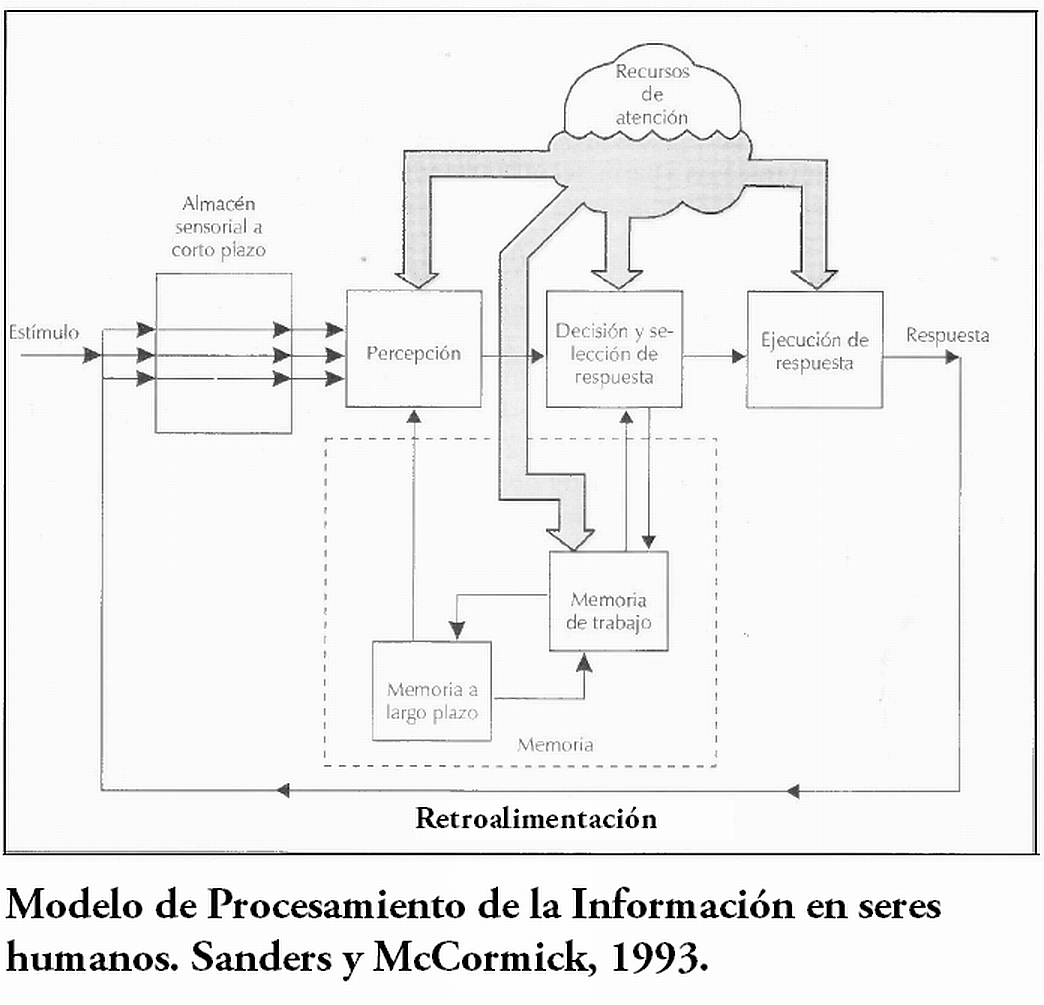
\includegraphics[width=0.6\linewidth]{imagenes/1.1.introduccion/modelo_procesamiento_informacion.png}

{\tiny Fuente: Romosquera, \url{https://commons.wikimedia.org/wiki/File:Procesamiento_de_la_Informaci\%C3\%B3n.png}
\\ \cite{mark1993human} }

\end{frame}

\begin{frame}{Ergonom\'ia F\'isica}
  
\end{frame}

\begin{frame}{Ergonom\'ia Visual}
  
\end{frame}



\begin{frame}

  \begin{columns}
    \begin{column}{0.45\textwidth}
      \begin{block}{Sistema de ciclo cerrado persona-m\'aquina}
        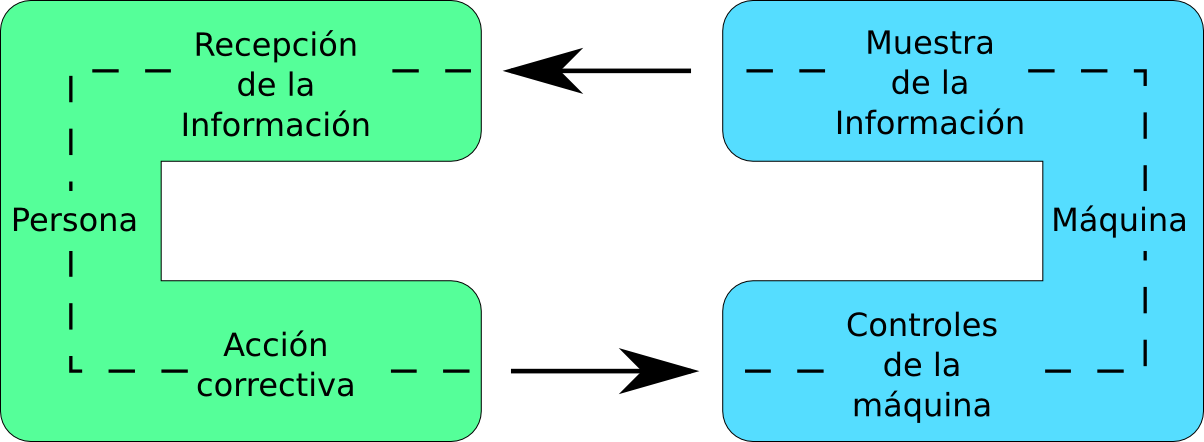
\includegraphics[width=\linewidth]{tikz/01-03-loop-persona-maquina.png}

        {\tiny Adaptado de \cite{bhandari2010design}}
      \end{block}
    \end{column}

    \begin{column}{0.05\textwidth}
    \end{column}

    \begin{column}{0.45\textwidth}

    \end{column}
      
  \end{columns}

\end{frame}
